\section{РУКОВОДСТВО ПОЛЬЗОВАТЕЛЯ}
\label{sec:manual}

\subsection{Требования к программному обеспечению}

Программа разработана для Google Colaboratory. Наличие возможности подключиться к вычислениям на GPU. В бесплатной версии есть ограничение на количество оперативной памяти графического процессора, но для запуска и комфортной работы хватит бесплатных мощностей.

\subsection{Руководство по установке}

Для работы с данной программой необходим интерпретатор Python 3.10.12, в Google Colaboratory, он установлен автоматически.

Для запуска модуля необходимо перейти на официальный сайт Google Colaboratory~\cite{colab} и загрузить файл в среду разработки.

После этого необходимо последовательно запускать команды и соглашаться со всеми всплывающими формами.

\begin{enumerate_num}
    \item Запустить команду \lstinline{!nvidia-smi} и убедиться что есть возможность использовать GPU.
    \item Выбрать GPU для вычислений.
    \item Загрузить все зависимости из раздела <<Dependencies>>.
    \item Разрешить Google Colaboratory доступ к Google Drive.
    \item Загрузить исходный код из раздела <<Source code>>.
\end{enumerate_num}

После этого можно непосредственно работать с модулем.

\subsection{Руководство по использованию}

\subsubsection{Редактирование изображения по текстовому описанию}

Первым делом необходимо скопировать изображение изображение из Google Drive в локальное хранилище блокнота:

\begin{lstlisting}[basicstyle=\ttfamily\small]
    !cp gdrive/MyDrive/Diplom/Images/Street.jpeg 
    /usr/share/jupyter/nbextensions/Street.jpeg
\end{lstlisting}

После необходимо указать путь до изображения которое было перемещенно в локальное хранилище и указать имя файла:

\begin{lstlisting}[basicstyle=\ttfamily\small]
    img_path = "/usr/local/share/jupyter/nbextensions/Street.jpg"
    original_filename = "Street.jpg"
\end{lstlisting}

Следующий шаг это инициализация объекта и загрузка зависимостей с указанием размера изображения, имени файла и других необходимых параметров:

\begin{lstlisting}[basicstyle=\ttfamily\small]
    diffusion_painter = DiffiusionPainter (original_filename=original_filename, canvas_w=600, canvas_h=400)
    diffusion_painter.prepare()
\end{lstlisting}

Вызов команды для начала изменения:

\begin{lstlisting}[basicstyle=\ttfamily\small]
    diffusion_painter.predict()
\end{lstlisting}

После этого будет выведено начальное окно работы с модулем представлено на рисунке~\ref{man::car_start}. На нём можно выбрать количество изображений которое будет сгенерирванно, масштаб изображения, количество шагов для генерации.

\begin{figure}[ht]
    \centering
    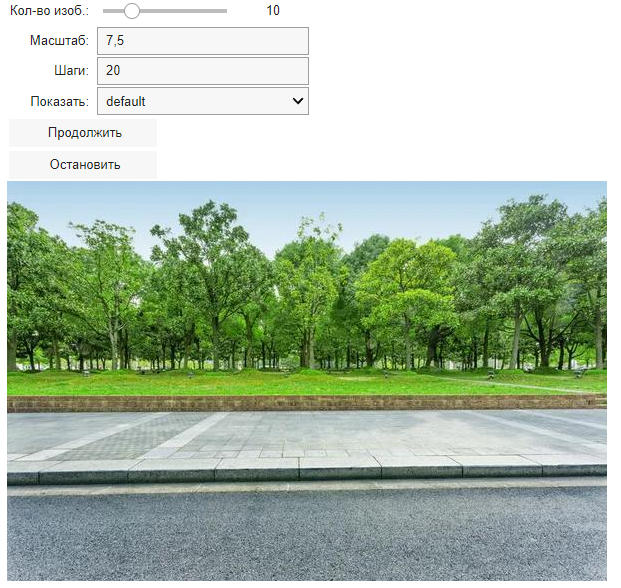
\includegraphics[width=.45\linewidth]{car_start.png}
    \caption{Начальная форма}
    \label{man::car_start}
\end{figure}

После выбора всех параметром и нажатия кнопки продолжить, форма меняется на другую, которая представлена на рисунке~\ref{man::car_select}. 

\begin{figure}[ht]
    \centering
    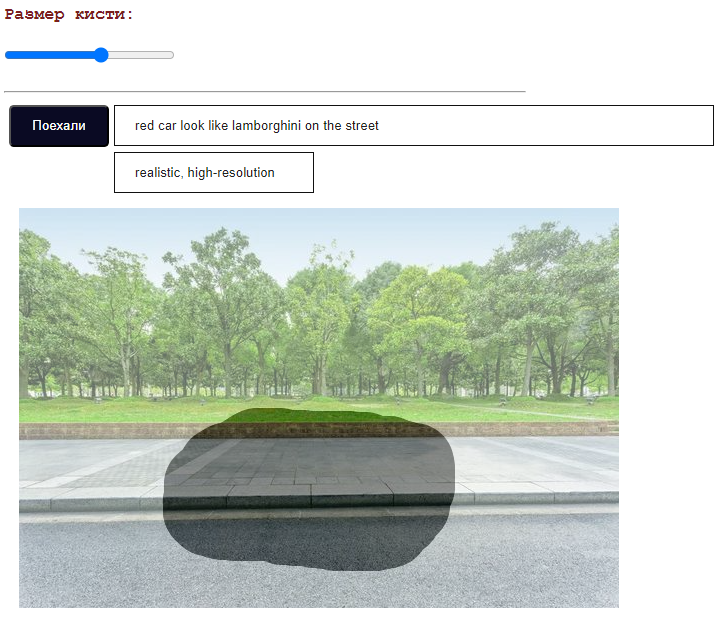
\includegraphics[width=.45\linewidth]{car_promt.png}
    \caption{Форма выбора области для изменения и написания текста}
    \label{man::car_select}
\end{figure}

Новая форма позволяет выбрать размер кисти которая позволяет выделить область на изображении для изменения и так же текстовое поле для написания промта для генерации. 

После будет показан прогресс бар и выделенная маска в которое будет генерировать изображение. После окончания генерации будет выведен результат, представленный на рисунке~\ref{man::car_end} нажав на dropdown <<Показать>> можно выбрать изображение и после нажатия кнопки <<Остановить>> изображение будет сохранено, или же можно нажать <<Продолжить>> и выбрать ещё области на изображении для изменения. 

\begin{figure}[ht]
    \centering
    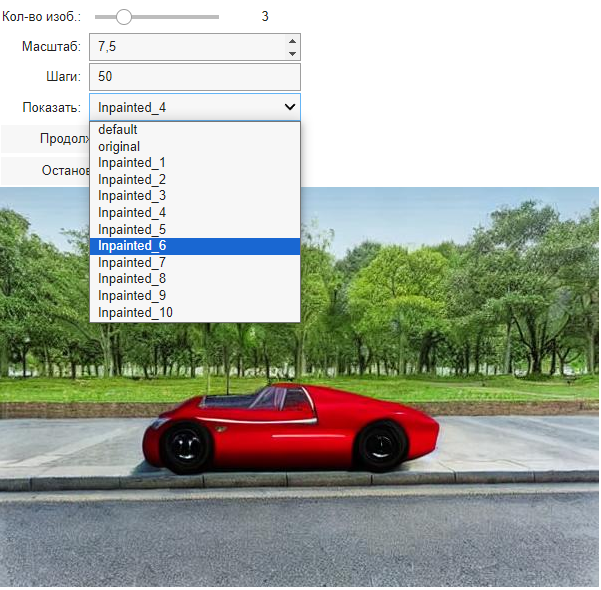
\includegraphics[width=.6\linewidth]{car_result.png}
    \caption{Финальная форма}
    \label{man::car_end}
\end{figure}

\subsubsection{Работа с масками изображения}

Разработанный программный модуль так же предоставляет несколько интересных функций и возможностей, которые расширяют гибкость и удобство использования. 

Помимо автоматической сегментации изображений, представленной на рисунке~\ref{dev::dog_all},  модуль предлагает альтернативный подход к сегментации - сегментацию по клику. Эта функция позволяет пользователю выбирать области на изображении, которые требуется включить в процесс сегментации, а также указывать области, которые не следует включать. Модель сегментации способна генерировать соответствующие маски на основе этих пользовательских точек. Это предоставляет пользователю большую гибкость и контроль над процессом сегментации.

Рассмотрим данную функциональность на примере редактирования комнатного интерьера. Исходный интерьер представлен на рисунке~\ref{man::flat}. 

\begin{figure}[ht]
    \centering
    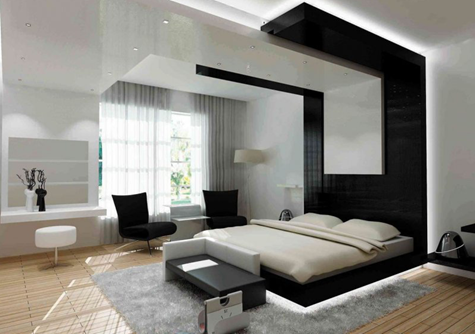
\includegraphics[width=.45\linewidth]{flat.png}
    \caption{Исходный интерьер квартиры}
    \label{man::flat}
\end{figure}

Можно заметить, что интерьер квартиры довольно приятный, однако текущие шторы не очень подходят к данному дизайну. Попробуем заменить их другим более приятным вариантом.

Выделим, как показано на рисунке~\ref{man::flat_points} область штор, которую хотим изменить с помощью диффузионной модели, а также области, которые не должны быть включены. Зеленые метки~-- области, которые хотим включить, красные~-- которые должны быть исключены из маски.

\begin{figure}[ht]
    \centering
    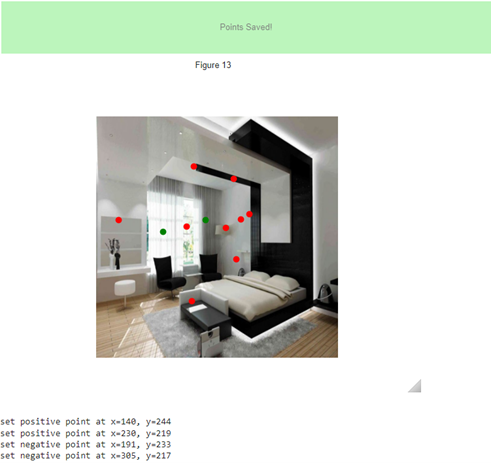
\includegraphics[width=.65\linewidth]{flat_points.png}
    \caption{Сегментирование изображения путем добавления хороших и плохих точек}
    \label{man::flat_points}
\end{figure}

Результат работы сегментирующей нейронной сети, на вход который помимо изображения были подана желательные и нежелательные точки для сегментации приведен на рисунке~\ref{manual::flat_seg_result}

\begin{figure}[ht]
    \centering
    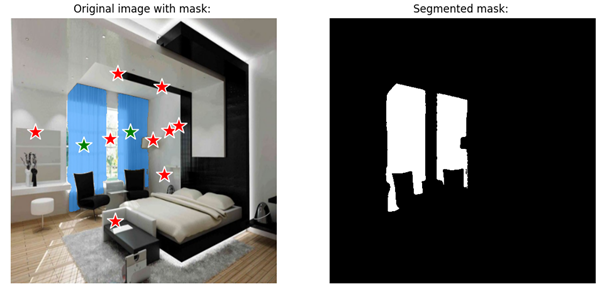
\includegraphics[width=.8\linewidth]{flat_segmentation.png}
    \caption{Результат выполненной сегментации с помощью точек}
    \label{manual::flat_seg_result}
\end{figure}

Произведем замену данных штор на более приятные с помощью диффузионной нейронной сети. К данной маске на вход подадим текст для желаемого результата: <<White pleasant lush curtains in the bedroom, realistic, high-resolution>>, результат представлен на рисунке~\ref{man::flat_result}. Как можно вид у комнаты преобразился в лучшую сторону. 

\begin{figure}[ht]
    \centering
    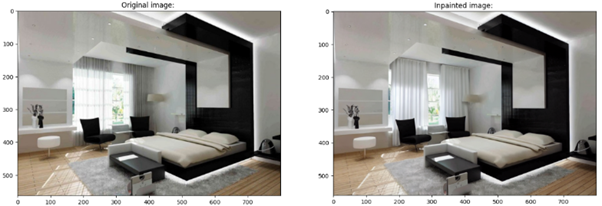
\includegraphics[width=1\linewidth]{flat_result.png}
    \caption{Новый интерьер с измененными шторами}
    \label{man::flat_result}
\end{figure}
